\documentclass{article}
\usepackage[hmargin=2.5cm]{geometry}
\usepackage{tikz}
\usepackage{verbatim}
\usetikzlibrary{calc, shadings, shadows, shapes.arrows}
\usetikzlibrary{shapes}
\usetikzlibrary{arrows}
\usetikzlibrary{positioning}
\usetikzlibrary{patterns}
\usetikzlibrary{calc}


\makeatletter
\pgfkeys{/pgf/.cd,
  parallelepiped offset x/.initial=2mm,
  parallelepiped offset y/.initial=2mm
}


\pgfdeclareshape{parallelepiped}
{
  \inheritsavedanchors[from=rectangle] % this is nearly a rectangle
  \inheritanchorborder[from=rectangle]
  \inheritanchor[from=rectangle]{north}
  \inheritanchor[from=rectangle]{north west}
  \inheritanchor[from=rectangle]{north east}
  \inheritanchor[from=rectangle]{center}
  \inheritanchor[from=rectangle]{west}
  \inheritanchor[from=rectangle]{east}
  \inheritanchor[from=rectangle]{mid}
  \inheritanchor[from=rectangle]{mid west}
  \inheritanchor[from=rectangle]{mid east}
  \inheritanchor[from=rectangle]{base}
  \inheritanchor[from=rectangle]{base west}
  \inheritanchor[from=rectangle]{base east}
  \inheritanchor[from=rectangle]{south}
  \inheritanchor[from=rectangle]{south west}
  \inheritanchor[from=rectangle]{south east}
  \backgroundpath{
    % store lower right in xa/ya and upper right in xb/yb
    \southwest \pgf@xa=\pgf@x \pgf@ya=\pgf@y
    \northeast \pgf@xb=\pgf@x \pgf@yb=\pgf@y
    \pgfmathsetlength\pgfutil@tempdima{\pgfkeysvalueof{/pgf/parallelepiped
      offset x}}
    \pgfmathsetlength\pgfutil@tempdimb{\pgfkeysvalueof{/pgf/parallelepiped
      offset y}}
    \def\ppd@offset{\pgfpoint{\pgfutil@tempdima}{\pgfutil@tempdimb}}
    \pgfpathmoveto{\pgfqpoint{\pgf@xa}{\pgf@ya}}
    \pgfpathlineto{\pgfqpoint{\pgf@xb}{\pgf@ya}}
    \pgfpathlineto{\pgfqpoint{\pgf@xb}{\pgf@yb}}
    \pgfpathlineto{\pgfqpoint{\pgf@xa}{\pgf@yb}}
    \pgfpathclose
    \pgfpathmoveto{\pgfqpoint{\pgf@xb}{\pgf@ya}}
    \pgfpathlineto{\pgfpointadd{\pgfpoint{\pgf@xb}{\pgf@ya}}{\ppd@offset}}
    \pgfpathlineto{\pgfpointadd{\pgfpoint{\pgf@xb}{\pgf@yb}}{\ppd@offset}}
    \pgfpathlineto{\pgfpointadd{\pgfpoint{\pgf@xa}{\pgf@yb}}{\ppd@offset}}
    \pgfpathlineto{\pgfqpoint{\pgf@xa}{\pgf@yb}}
    \pgfpathmoveto{\pgfqpoint{\pgf@xb}{\pgf@yb}}
    \pgfpathlineto{\pgfpointadd{\pgfpoint{\pgf@xb}{\pgf@yb}}{\ppd@offset}}
  }
}
\makeatother



\tikzstyle{pc1}   = [
parallelepiped, 
minimum width=12pt, 
text width=12pt, 
inner sep=12pt, 
draw, 
line width=2pt, 
path picture=
	{
	\draw (-1,-1) -- ++(1,-2);
	}
]




\tikzset{
  ports/.style={
    line width=0.3pt,
    top color=gray!20,
    bottom color=gray!20
  },
  rack switch/.style={
    parallelepiped,fill=white, draw,
    minimum width=1.25cm,
    minimum height=0.25cm,
    parallelepiped offset x=2mm,
    parallelepiped offset y=1.25mm,
    xscale=-1,
    path picture={
      \draw[top color=gray!5,bottom color=gray!40]
      (path picture bounding box.south west) rectangle 
      (path picture bounding box.north east);
      \coordinate (A-west) at ([xshift=-0.2cm]path picture bounding box.west);
      \coordinate (A-center) at ($(path picture bounding box.center)!0!(path
        picture bounding box.south)$);
      \foreach \x in {0.275,0.525,0.775}{
        \draw[ports]([yshift=-0.05cm]$(A-west)!\x!(A-center)$)
          rectangle +(0.1,0.05);
        \draw[ports]([yshift=-0.125cm]$(A-west)!\x!(A-center)$)
          rectangle +(0.1,0.05);
       } 
      \coordinate (A-east) at (path picture bounding box.east);
      \foreach \x in {0.085,0.21,0.335,0.455,0.635,0.755,0.875,1}{
        \draw[ports]([yshift=-0.1125cm]$(A-east)!\x!(A-center)$)
          rectangle +(0.05,0.1);       
      }
    }
  },
  server/.style={
    parallelepiped,
    fill=white, draw,
    minimum width=0.35cm,
    minimum height=0.75cm,
    parallelepiped offset x=3mm,
    parallelepiped offset y=3mm,
    xscale=-1,
    path picture={
      \draw[top color=gray!5,bottom color=gray!40]
      (path picture bounding box.south west) rectangle 
      (path picture bounding box.north east);
      \coordinate (A-center) at ($(path picture bounding box.center)!0!(path
        picture bounding box.south)$);
      \coordinate (A-west) at ([xshift=-0.575cm]path picture bounding box.west);
      \draw[ports]([yshift=0.1cm]$(A-west)!0!(A-center)$)
        rectangle +(0.2,0.065);
      \draw[ports]([yshift=0.01cm]$(A-west)!0.085!(A-center)$)
        rectangle +(0.15,0.05);
      \fill[black]([yshift=-0.35cm]$(A-west)!-0.1!(A-center)$)
        rectangle +(0.235,0.0175);
      \fill[black]([yshift=-0.385cm]$(A-west)!-0.1!(A-center)$)
        rectangle +(0.235,0.0175);
      \fill[black]([yshift=-0.42cm]$(A-west)!-0.1!(A-center)$)
        rectangle +(0.235,0.0175);
    }  
  }
}



% Styles for interfaces and edge labels
\tikzset{%
  interface/.style={draw, rectangle, rounded corners, font=\LARGE\sffamily},
  ethernet/.style={interface, fill=yellow!50},% ethernet interface
  serial/.style={interface, fill=green!70},% serial interface
  speed/.style={sloped, anchor=south, font=\large\sffamily},% line speed at edge
  route/.style={draw, shape=single arrow, single arrow head extend=4mm,
    minimum height=1.7cm, minimum width=3mm, white, fill=white!20,
    drop shadow={opacity=.8, fill=white!50!black}, font=\tiny}% inroute / outroute arrows
}
\newcommand*{\shift}{1.3cm}% For placing the arrows later



\newcommand*{\laptop}{
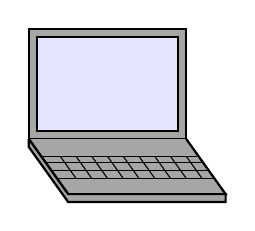
\begin{tikzpicture}    
%backmonitor
\draw[thick, fill=gray!70] (0,0) rectangle (2,1.4);

%screen
\draw[thick, fill=blue!10] (0.1,0.1) rectangle (1.9,1.3);

%keyboard
\draw[thick, fill=gray!70] (0,0) -- (.5,-.7) -- (2.5,-.7) -- (2,0);
\draw[thick, fill=gray!70] (0,0) -- (0,-.1) -- (.5,-0.8) -- (2.5,-.8) -- (2.5,-.7) -- (.5,-0.7) -- (0,0);
\foreach \x in {.4,.6,.8,1,1.2,1.4,1.6,1.8,2} {
\draw (\x,-.22) -- (\x+.2,-.5);
}
\draw (.14,-.12-.1) -- (2+.14,-.12-.1);
\draw (.2,-.2-.1) -- (2+.2,-.2-.1);
\draw (.3,-.3-.1) -- (2+.3,-.3-.1);
\draw (.37,-.4-.1) -- (2+.37,-.4-.1);
%\foreach \x in {.12,.2,.3,.4} {
%\draw (\x,-\x-.1) -- (2+\x,-\x-.1);
%}
\end{tikzpicture}
}




\newcommand*{\computer}{
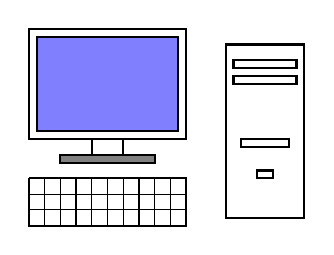
\begin{tikzpicture}   
%back monitor 
\draw[thick] (0,0) rectangle (2,1.4);
%\draw[thick] (0,1.4) -- (.1,1.5) -- (2.1,1.5) -- (2,1.4);
%\draw[thick] (2.1,1.5) -- (2.1,.1) -- (2,0);

%screen
\draw[thick, fill=blue!50] (0.1,0.1) rectangle (1.9,1.3);


%monitor LEG
\draw[thick] (.8,0) rectangle (1.2,-.2);
\draw[thick, fill=gray] (.4,-.2) rectangle (1.6,-.3);

%keyboard
\draw[thick] (0,-0.5) -- (0,-1.1) -- (2,-1.1) -- (2,-0.5) --(0,-0.5);
\foreach \x in {.2,.4,.6,.8,1,1.2,1.4,1.6,1.8} {
\draw (\x,-0.5) -- (\x,-1.1);
}
\foreach \x in {-.5,.-.7,-.9} {
\draw (0,\x) -- (2,\x);
}

%case
\draw[thick] (2.5,-1) rectangle (3.5,1.2);
\draw[thick] (2.6,.7) rectangle (3.4,.8);
\draw[thick] (2.6,.9) rectangle (3.4,1);
\draw[thick] (2.7,-.1) rectangle (3.3,0);
\draw[thick] (2.9,-.5) rectangle (3.1,-.4);

\end{tikzpicture}
}











\newcommand*{\computertwo}{
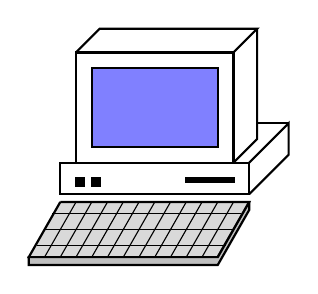
\begin{tikzpicture}   
%back monitor 
\draw[thick] (0,0) rectangle (2,1.4);
\draw[thick] (0,1.4) -- (.3,1.7) -- (2.3,1.7) -- (2,1.4);
\draw[thick] (2.3,1.7) -- (2.3,.3) -- (2,0);

%screen
\draw[thick, fill=blue!50] (0.2,0.2) rectangle (1.8,1.2);


%monitor LEG
\draw[thick] (-.2,0) rectangle (2.2,-.4);
\draw[thick] (2.2,0) -- (2.7,.5) -- (2.7,.1) -- (2.2,-.4) ;
\draw[thick] (2.7,.5) -- (2.3,.5);
%\draw[thick, fill=gray] (.4,-.2) rectangle (1.6,-.3);


%keyboard
\draw[thick, fill=gray!30] (-0.2,-.5) -- (2.2,-.5) -- (1.8,-1.2) -- (-.6,-1.2) -- (-0.2,-.5) ;
\draw[thick, fill=gray!50] (2.2,-.5) -- (2.2,-.6) -- (1.8,-1.3) --  (-.6,-1.3) -- (-.6,-1.2) -- (1.8,-1.2) -- (2.2,-.5) ;

%\draw (0,-.7) rectangle (.1,-.8);
\foreach \x in {0,.2,.4,.6,.8,1,1.2,1.4,1.6,1.8,2} {
\draw (\x,-0.5) -- (\x-.4,-1.2);
}
\draw (-0.3,-.65) -- (2.1,-.65);
\draw (-0.4,-.85) -- (2,-.85);
\draw (-0.5,-1.05) -- (1.9,-1.05);
%\foreach \x in {-.7,-.9,-1.1} {
%\draw (-0.3,\x) -- (2+0.2,\x);
%}


\draw[thick, fill=black] (0,-.2) rectangle (0.1,-.3);
\draw[thick, fill=black] (0.2,-.2) rectangle (0.3,-.3);

\draw[thick, fill=black] (1.4,-.2) rectangle (2,-.25);

\end{tikzpicture}
}















\newcommand*{\computerthree}{
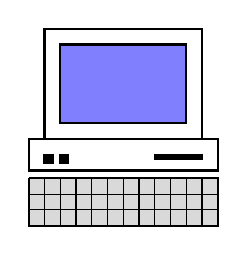
\begin{tikzpicture}   
%back monitor 
\draw[thick] (0,0) rectangle (2,1.4);
%\draw[thick] (0,1.4) -- (.3,1.7) -- (2.3,1.7) -- (2,1.4);
%\draw[thick] (2.3,1.7) -- (2.3,.3) -- (2,0);

%screen
\draw[thick, fill=blue!50] (0.2,0.2) rectangle (1.8,1.2);


%monitor LEG
\draw[thick] (-.2,0) rectangle (2.2,-.4);
%\draw[thick] (2.2,0) -- (2.7,.5) -- (2.7,.1) -- (2.2,-.4) ;
%\draw[thick] (2.7,.5) -- (2.3,.5);
%\draw[thick, fill=gray] (.4,-.2) rectangle (1.6,-.3);


%keyboard
\draw[thick, fill=gray!30] (-0.2,-.5) -- (2.2,-.5) -- (2.2,-1.1) -- (-0.2,-1.1) -- (-0.2,-.5) ;
%\draw[thick, fill=gray!50] (2.2,-.5) -- (2.2,-.6) -- (1.8,-1.3) --  (-.6,-1.3) -- (-.6,-1.2) -- (1.8,-1.2) -- (2.2,-.5) ;

%\draw (0,-.7) rectangle (.1,-.8);
\foreach \x in {0,.2,.4,.6,.8,1,1.2,1.4,1.6,1.8,2} {
\draw (\x,-0.5) -- (\x,-1.1);
}
\draw (-0.2,-.7) -- (2.2,-.7);
\draw (-0.2,-.9) -- (2.2,-.9);
\draw (-0.2,-1.1) -- (2.2,-1.1);
%\foreach \x in {-.7,-.9,-1.1} {
%\draw (-0.3,\x) -- (2+0.2,\x);
%}


\draw[thick, fill=black] (0,-.2) rectangle (0.1,-.3);
\draw[thick, fill=black] (0.2,-.2) rectangle (0.3,-.3);
\draw[thick, fill=black] (1.4,-.2) rectangle (2,-.25);

\end{tikzpicture}
}









% The router icon
\newcommand*{\router}[1]{
\begin{tikzpicture}[xscale=.4,yscale=.6] 
  \coordinate (ll) at (-3,0.5);
  \coordinate (lr) at (3,0.5);
  \coordinate (ul) at (-3,2);
  \coordinate (ur) at (3,2);
  \shade [shading angle=90, left color=black!40!white, right color=white] ($(ll)+(0,.5)$) arc (-180:-60:3cm and .75cm) -- +(0,1) arc (-60:-180:3cm and .75cm)
    -- cycle;
  \shade [shading angle=270, right color=black!40!white, left color=white!50] ($(lr)+(0,.5)$) arc (0:-60:3cm and .75cm) -- +(0,1) arc (-60:0:3cm and .75cm) -- cycle;
  \draw [thick] ($(ll)+(0,.5)$) arc (-180:0:3cm and .75cm) -- (ur) arc (0:-180:3cm and .75cm)
    -- cycle;
  \draw [thick, shade, upper left=white!30!black, lower left=white!80!white, upper right=white!80!white, lower right=white] (ul) arc (-180:180:3cm and .75cm);
  \node at (0,0.5){\color{blue!60!black}\Huge #1};% The name of the router
  % The four arrows, symbols for incoming and outgoing routes:
  \begin{scope}[yshift=2cm, yscale=0.28, transform shape]
    \node[route, rotate=45, xshift=\shift] {\strut};
    \node[route, rotate=-45, xshift=-\shift] {\strut};
    \node[route, rotate=-135, xshift=\shift] {\strut};
    \node[route, rotate=135, xshift=-\shift] {\strut};
  \end{scope}
\end{tikzpicture}}

\begin{document}
\pagestyle{empty}

\begin{comment}
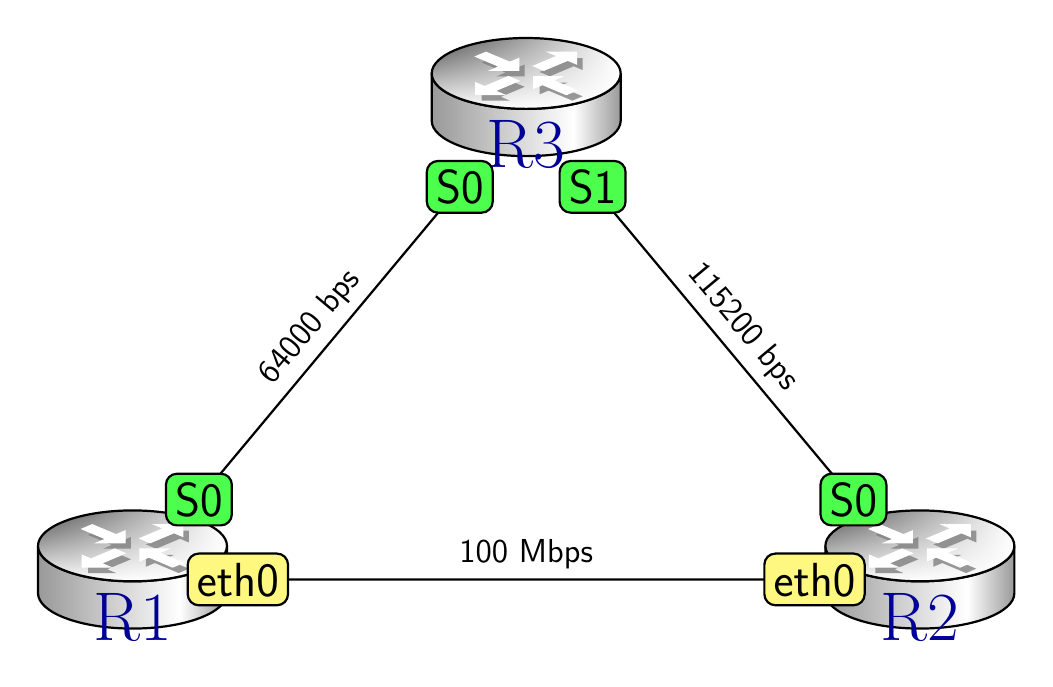
\begin{tikzpicture}[node distance=10cm]
  % Place three routers as nodes:
  \node (R1) {\router{R1}};
  \node [right of=R1] (R2) {\router{R2}};
  \node[yshift=6cm] at ($ (R1) !.5! (R2) $)  (R3) {\router{R3}};
  % Connect by lines and specify interfaces and speed:
  \draw[thick] (R1)
    -- node[ethernet,  at start]{eth0} node[ethernet, at end] {eth0} (R2)
      node[speed,midway] {100 Mbps}
    -- node[serial,  at start]{S0} node[serial, at end] {S1} (R3)
      node[speed,midway] {115200 bps}
    -- node[serial,  at start]{S0} node[serial, at end] {S0} (R1)
      node[speed,midway] {64000 bps};
\end{tikzpicture}
\end{comment}


\begin{center}
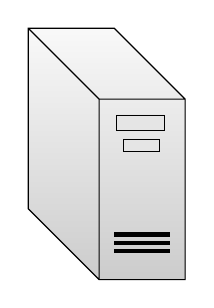
\begin{tikzpicture}
  \node[scale=3,server] (R1) {};
\end{tikzpicture}
\end{center}


\begin{center}
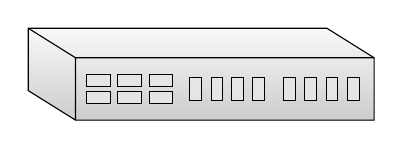
\begin{tikzpicture}
  \node[scale=3,rack switch] (R1) {};
\end{tikzpicture}
\end{center}



\begin{center}
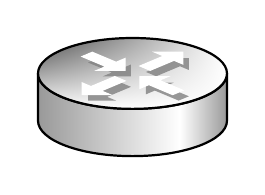
\begin{tikzpicture}
  \node (R1) {\router{}};
\end{tikzpicture}
\end{center}


\begin{center}

\begin{tikzpicture}
  \node (R1) {\laptop};
\end{tikzpicture}
\end{center}


\begin{center}
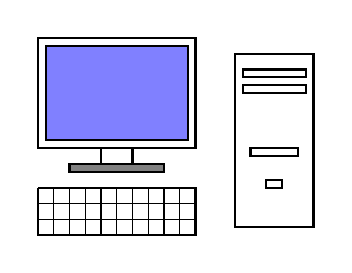
\begin{tikzpicture}
  \node (R1) {\computer};
\end{tikzpicture}
\end{center}


\begin{center}
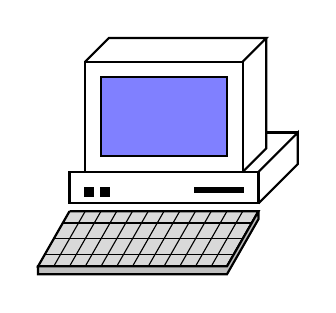
\begin{tikzpicture}
  \node (R1) {\computertwo};
\end{tikzpicture}
\end{center}



\begin{center}
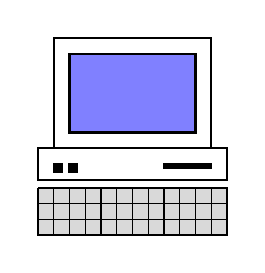
\begin{tikzpicture}
  \node (R1) {\computerthree};
\end{tikzpicture}
\end{center}



\begin{center}
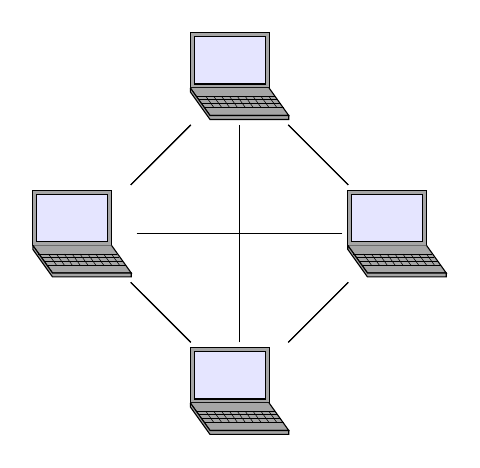
\begin{tikzpicture}
  \node[scale=0.5] (a) at (0,0) {\laptop};
  \node[scale=0.5] (b) at (2,2) {\laptop};
  \node[scale=0.5] (c) at (4,0) {\laptop};
  \node[scale=0.5] (d) at (2,-2) {\laptop};
  \foreach \from in {a,b,c,d} {
  	\foreach \to in {a,b,c,d} {
	    \draw (\from) -- (\to);
	}
  }
\end{tikzpicture}
\end{center}







\begin{center}
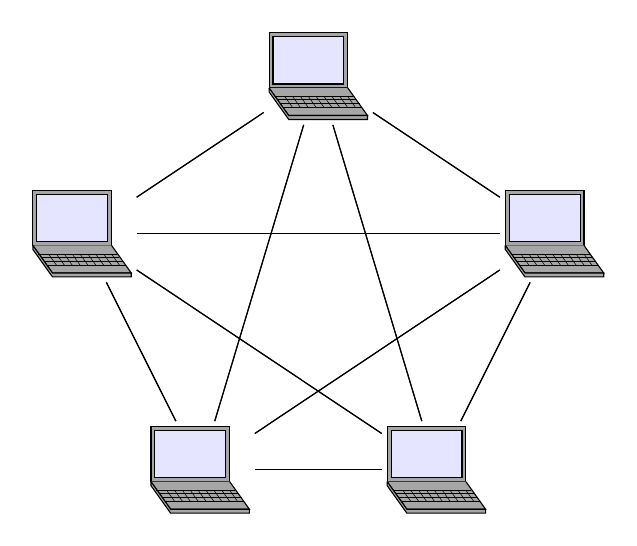
\begin{tikzpicture}
  \node[scale=0.5] (a) at (0,0) {\laptop};
  \node[scale=0.5] (b) at (1.5,-3) {\laptop};
  \node[scale=0.5] (c) at (4.5,-3) {\laptop};
  \node[scale=0.5] (d) at (6,0) {\laptop};
  \node[scale=0.5] (e) at (3,2) {\laptop};
  \foreach \from in {a,b,c,d,e} {
  	\foreach \to in {a,b,c,d,e} {
	    \draw (\from) -- (\to);
	}
  }
\end{tikzpicture}
\end{center}








\begin{center}
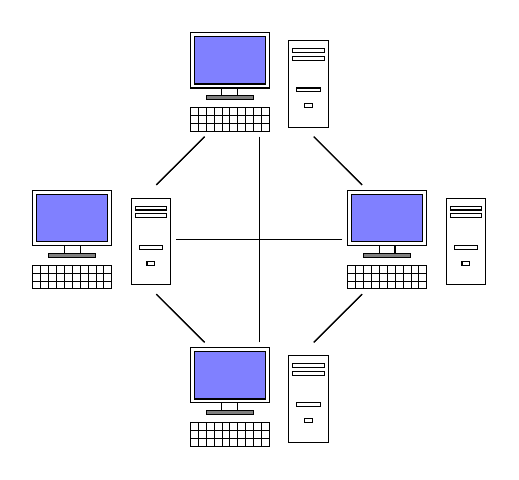
\begin{tikzpicture}
  \node[scale=0.5] (a) at (0,0) {\computer};
  \node[scale=0.5] (b) at (2,2) {\computer};
  \node[scale=0.5] (c) at (4,0) {\computer};
  \node[scale=0.5] (d) at (2,-2) {\computer};
  \foreach \from in {a,b,c,d} {
  	\foreach \to in {a,b,c,d} {
	    \draw (\from) -- (\to);
	}
  }
\end{tikzpicture}
\end{center}







\begin{center}
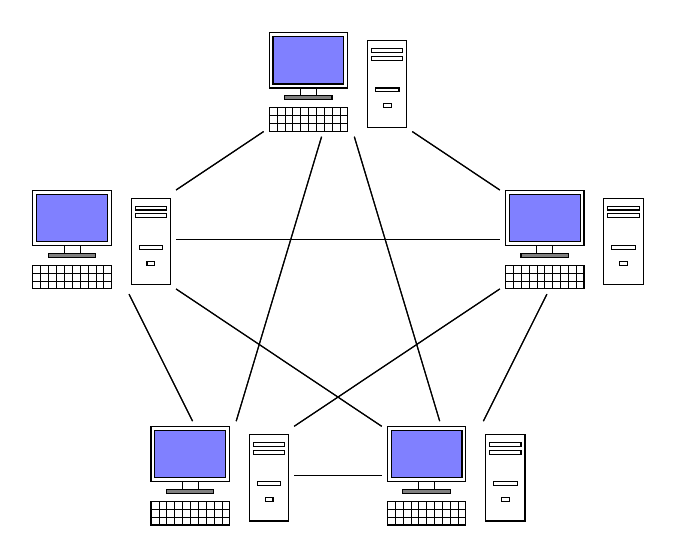
\begin{tikzpicture}
  \node[scale=0.5] (a) at (0,0) {\computer};
  \node[scale=0.5] (b) at (1.5,-3) {\computer};
  \node[scale=0.5] (c) at (4.5,-3) {\computer};
  \node[scale=0.5] (d) at (6,0) {\computer};
  \node[scale=0.5] (e) at (3,2) {\computer};
  \foreach \from in {a,b,c,d,e} {
  	\foreach \to in {a,b,c,d,e} {
	    \draw (\from) -- (\to);
	}
  }
\end{tikzpicture}
\end{center}











\begin{center}
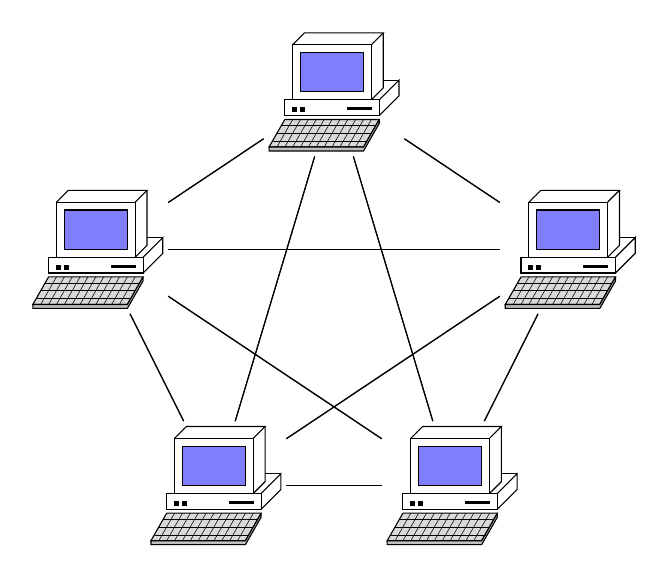
\begin{tikzpicture}
  \node[scale=0.5] (a) at (0,0) {\computertwo};
  \node[scale=0.5] (b) at (1.5,-3) {\computertwo};
  \node[scale=0.5] (c) at (4.5,-3) {\computertwo};
  \node[scale=0.5] (d) at (6,0) {\computertwo};
  \node[scale=0.5] (e) at (3,2) {\computertwo};
  \foreach \from in {a,b,c,d,e} {
  	\foreach \to in {a,b,c,d,e} {
	    \draw (\from) -- (\to);
	}
  }
\end{tikzpicture}
\end{center}







\begin{center}
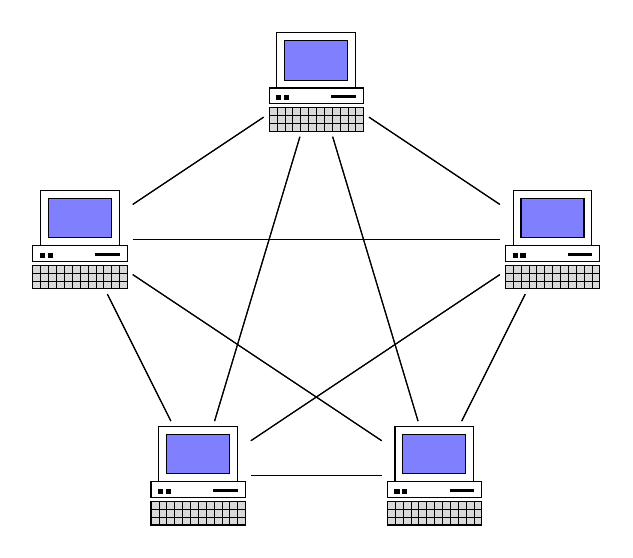
\begin{tikzpicture}
  \node[scale=0.5] (a) at (0,0) {\computerthree};
  \node[scale=0.5] (b) at (1.5,-3) {\computerthree};
  \node[scale=0.5] (c) at (4.5,-3) {\computerthree};
  \node[scale=0.5] (d) at (6,0) {\computerthree};
  \node[scale=0.5] (e) at (3,2) {\computerthree};
  \foreach \from in {a,b,c,d,e} {
  	\foreach \to in {a,b,c,d,e} {
	    \draw (\from) -- (\to);
	}
  }
\end{tikzpicture}
\end{center}





\end{document}